\begin{frame}
    \frametitle{Simulations: Aim}
    Compare in the first stage (selection equation) the approaches:
    \begin{itemize}
        \item Probit with dummies for fixed effects
        \item Probit with dummies for fixed effects correcting for perfect prediction 
        \item Charbonneau \\~\\ 
    \end{itemize}
    Compare in the second stage (observation equation) the approaches:
    \begin{itemize}
        \item Standard Heckman 
        \item Standard Heckman correcting for perfect prediction 
        \item Hybrid + Lee's transformation
        \item Modified Kyriazidou \\~\\ 
    \end{itemize}
    Assume that there is no misspecification in the distributional assumptions and in the parametric form of models. 
    \\~\\ 
    500 Monte Carlo simulations, sample size of $N=25$, yielding $(N(N-1))=600$ observations.
\end{frame}

\begin{frame}
    \frametitle{Simulations: DGP Designs}
    Considering only one time period:
    \begin{gather}
        y_{1,ij} = x_{1,ij}\beta_{11} + x_{2,ij}\beta_{12} + \vartheta_i + \chi_j + u_{ij} \nonumber\\
        y_{2,i j}= \mathbbm{1} (y_{2,i j}^{**} > 0) \nonumber\\
        y_{2,i j}^{**}=x_{1,ij}{\beta_{21}^*} + x_{2,ij}{\beta_{22}^*} + x_{3,ij}{\beta_{23}^*}  +\xi_{i}^*+\zeta_{j}^*+\eta^*_{i j} \nonumber
      \end{gather}
      \begin{equation*}
        \hspace{10000pt minus 1fil} (i = 1,...N; j=1,...N, i \neq j)\hfilneg
      \end{equation*}
      Set: $\beta_{11} = 1$, $\beta_{12} = 2.5$, $\beta_{21}^* = 0.8$, $\beta_{22}^* = 1$ and $\beta_{23}^* = 2$. \pause
      \\~\\ 
      \textbf{Design 5:} $\vartheta_i = \chi_j = 0$, $\xi_{i}^*$ and $\zeta_{j}^*$ drawn from standard normal distribution. \\
      \begin{itemize}
        \item $x_1 = \textit{rndn} + \xi_{i}^*+\zeta_{j}^*$, where $\textit{rndn}$ is a standard normal.
        \item $x_2 = \mathbbm{1}\{\textit{rndn} \leq 0.5\}$, being a bivariate variable.
        \item $x_3 = \mathbbm{1}\{\textit{rndn} \leq 0.5\}$, being a bivariate variable.
      \end{itemize}
      \textbf{Design 6:} $\xi_{i}^*=\zeta_{j}^*=0$, $\vartheta_i$ and $\chi_j$ drawn from standard normal distribution. $x_1 = \textit{rndn} + \vartheta_{i}+\chi_{j}$.
      \\~\\
      \textbf{Design 7:} All fixed effects and $x_1 = \textit{rndn} + \vartheta_{i}+\chi_{j} + \xi_{i}^*+\zeta_{j}^*$.
\end{frame}

\begin{frame}
    \frametitle{Simulations: First stage \textit{t-tests} for structural parameters}
    \begin{figure}
        \centerline{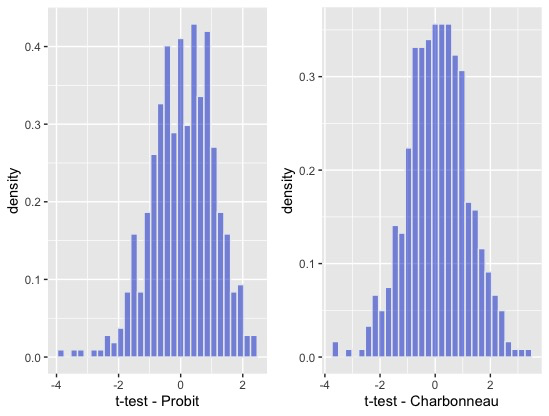
\includegraphics[scale=0.35]{content/Figures/ttest_beta21_Design6.png}}
        \caption{\footnotesize{Histogram of the \textit{t-test} for estimated $\beta_{21}^*$ in Design 6}}
        \label{ttest_beta21_Design6}
      \end{figure}
    Design that do not contain fixed effects in selection equation both approaches deliver similar results: distributions are centered around zero.
\end{frame}

\begin{frame}
    \frametitle{Simulations: First stage \textit{t-tests} for structural parameters}
    \begin{figure}
        \centerline{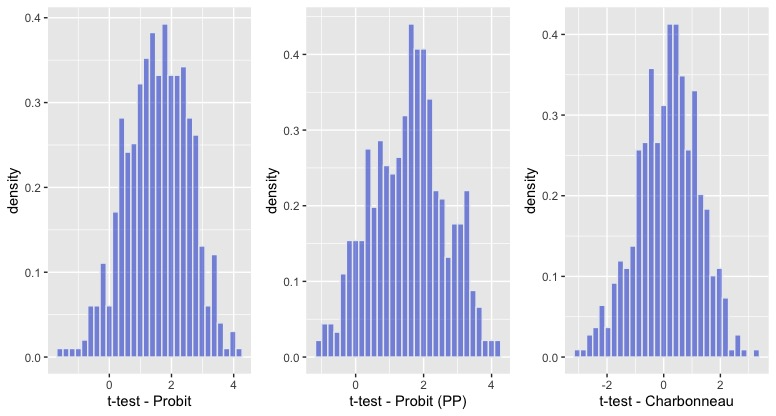
\includegraphics[scale=.35]{content/Figures/ttest_beta21_Design5.png}}
        \caption{\footnotesize{Histogram of the \textit{t-test} for estimated $\beta_{21}^*$ in Design 5}}
        \label{ttest_beta21_Design5}
      \end{figure}
\end{frame}

\begin{frame}
    \frametitle{Simulations: First stage \textit{t-tests} for structural parameters}
    \begin{figure}
        \centerline{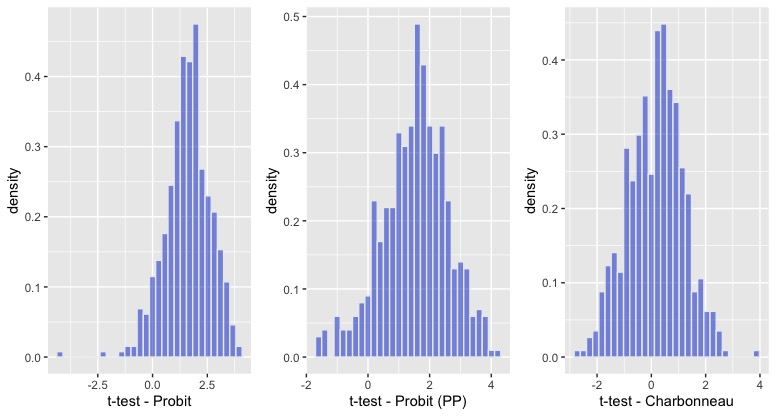
\includegraphics[scale=.35]{content/Figures/ttest_beta21_Design7.png}}
        \caption{\footnotesize{Histogram of the \textit{t-test} for estimated $\beta_{21}^*$ in Design 7}}
        \label{ttest_beta21_Design7}
      \end{figure}
      For Charbonneau, \textit{t-tests} are centered around zero, but not for Probit and Probit (PP). Biases of estimates for Probit and Probit (PP) are of the same magnitude $\xrightarrow{}$ reflects mostly incidental parameter problem.
\end{frame}

\begin{frame}
    \frametitle{Simulations: First stage QQ-plot for structural parameters}
    \begin{figure}
        \centerline{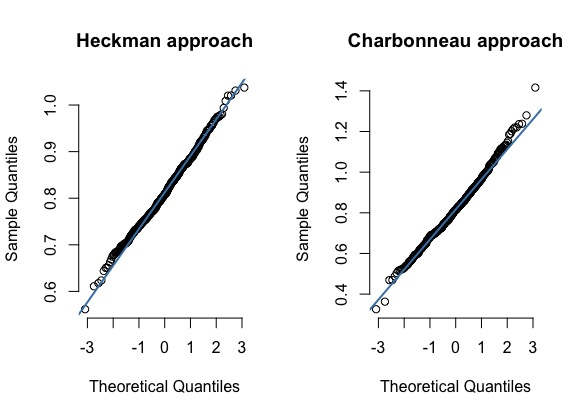
\includegraphics[scale=.35]{content/Figures/QQ_beta_21_Design6.png}}
        \caption{\footnotesize{QQ plot of estimated $\beta_{21}^*$ in Design 6}}
        \label{QQ_beta_21_Design6}
      \end{figure}
      All distributions are reasonably well approximated by a normal distribution.
\end{frame}

\begin{frame}
    \frametitle{Simulations: First stage QQ-plot for structural parameters}
    \begin{figure}
        \centerline{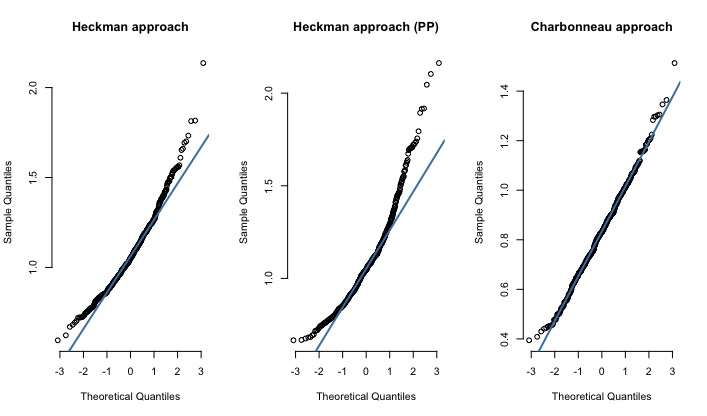
\includegraphics[scale=.35]{content/Figures/QQ_beta_21_Design5.png}}
        \caption{\footnotesize{QQ plot of estimated $\beta_{21}^*$ in Design 5}}
        \label{QQ_beta_21_Design5}
      \end{figure}
\end{frame}

\begin{frame}
    \frametitle{Simulations: First stage QQ-plot for structural parameters}
    \begin{figure}
        \centerline{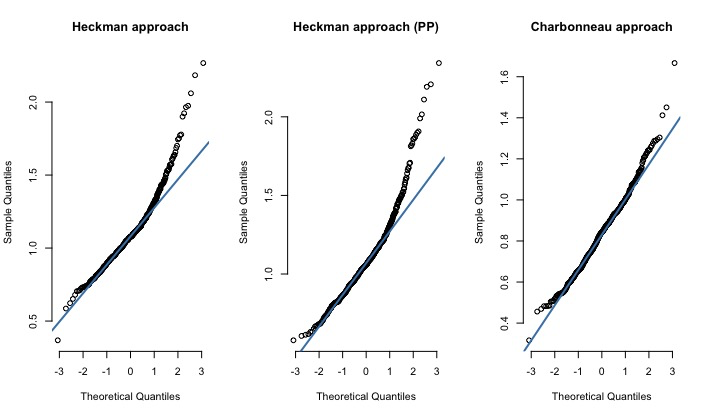
\includegraphics[scale=.35]{content/Figures/QQ_beta_21_Design7.png}}
        \caption{\footnotesize{QQ plot of estimated $\beta_{21}^*$ in Design 7}}
        \label{QQ_beta_21_Design7}
      \end{figure}
      In designs 5 and 7, Charbonneau are better approximated by a normal distribution. Other estimators are more skewed.
\end{frame}

\begin{frame}
    \frametitle{Simulations: First stage fixed effects}
    \begin{figure}
        \centerline{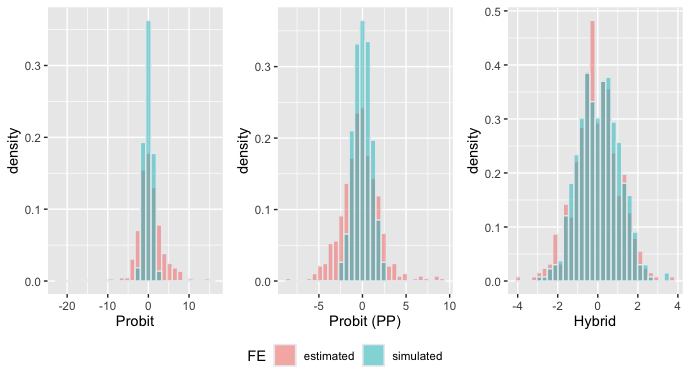
\includegraphics[scale=.35]{content/Figures/Hist_FE_Design5.png}}
        \caption{\footnotesize{Histogram of estimated $\xi_1^*$ in Design 5}}
        \label{fig}
      \end{figure}
\end{frame}

\begin{frame}
    \frametitle{Simulations: First stage fixed effects}
    \begin{figure}
        \centerline{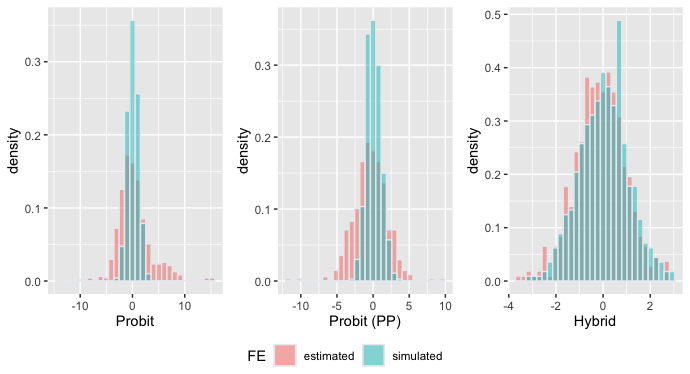
\includegraphics[scale=.35]{content/Figures/Hist_FE_Design7.png}}
        \caption{\footnotesize{Histogram of estimated $\xi_1^*$ in Design 7}}
        \label{fig}
      \end{figure}
      Probit estimates off due to: (i) not corrected for perfect prediction, and (ii) estimates are contaminated by the (asymptotic) bias of structural parameters.
      \hyperlink{single indices}{\beamerbutton{Results of single indices}}
\end{frame}

\begin{frame}
    \frametitle{Simulations: Second stage structural parameters mean bias}
    \begin{minipage}{7cm}
    \begin{figure}[htbp]
      \centerline{\includegraphics[scale=.28]{content/Figures/bias_beta11_design6.eps}}
      \caption{\footnotesize{Mean bias of  $\hat{\beta}_{11}$ in Design 6}}
      \label{bias_beta11_design6}
    \end{figure}
    \begin{figure}[htbp]
      \vspace{-2.5em}%
      \centerline{\includegraphics[scale=.28]{content/Figures/bias_beta12_design6.eps}}
      \caption{\footnotesize{Mean bias of  $\hat{\beta}_{12}$ in Design 6}}
      \label{bias_beta12_design6}
    \end{figure}
  \end{minipage}%
  \begin{minipage}{5cm}
             For the modified Kyriazidou: $r=1$ and $K$ set to be a standard normal density.\\~\\
             With no fixed effects, all proposed estimators have essentially no bias. \\~\\
             Even when including dummies in observation equations, estimators have nice properties. 
            \end{minipage}
  \end{frame}

  \begin{frame}
    \frametitle{Simulations: Second stage structural parameters mean bias}
    \begin{minipage}{7cm}
    \begin{figure}[htbp]
      \centerline{\includegraphics[scale=.28]{content/Figures/bias_beta11_design5.eps}}
      \caption{\footnotesize{Mean bias of  $\hat{\beta}_{11}$ in Design 5}}
      \label{bias_beta11_design5}
    \end{figure}
    \begin{figure}[htbp]
      \vspace{-2.5em}%
      \centerline{\includegraphics[scale=.28]{content/Figures/bias_beta12_design5.eps}}
      \caption{\footnotesize{Mean bias of  $\hat{\beta}_{12}$ in Design 5}}
      \label{bias_beta12_design5}
    \end{figure}
  \end{minipage}%
  \begin{minipage}{5cm}
    Heckman and Heckman(PP) have biases: single indices are biased.\\~\\
  \end{minipage}
  \end{frame}

  \begin{frame}
    \frametitle{Simulations: Second stage structural parameters mean bias}
    \begin{minipage}{7cm}
    \begin{figure}[htbp]
      \centerline{\includegraphics[scale=.28]{content/Figures/bias_beta11_design7.eps}}
      \caption{\footnotesize{Mean bias of  $\hat{\beta}_{11}$ in Design 7}}
      \label{bias_beta11_design7}
    \end{figure}
    \begin{figure}[htbp]
      \vspace{-2.5em}%
      \centerline{\includegraphics[scale=.28]{content/Figures/bias_beta12_design7.eps}}
      \caption{\footnotesize{Mean bias of  $\hat{\beta}_{12}$ in Design 7}}
      \label{bias_beta12_design7}
    \end{figure}
  \end{minipage}%
  \begin{minipage}{5cm}
    Kyriazidou reduces further the bias for the continuous variable.\\~\\
    Hybrid reduces further for the binary variable. \\~\\
    Estimates sensitive to initial choice of $h$.\\
    \hyperlink{qqplots}{\beamerbutton{QQ plots}}
  \end{minipage}
  \end{frame}



